\origpage{51}{GRAPH MINORS}
\sectionhead{3. \textsc{The Main Theorem}}

In order to prove our main theorem (1.1), it is only necessary to prove a
special case, as we shall now see. Let $\mathbf{Y}_1$ be the complete bipartite graph
$K_{1,3}$. For $\lambda\ge 2$, we define $\mathbf{Y}_\lambda$ inductively by taking a copy of $\mathbf{Y}_{\lambda-1}$, and to
each vertex of valency 1 in this graph making adjacent two new vertices.
(See Fig. 1.)

In order to prove (1.1), it is only necessary to prove the following:
\stmt
(3.1). \textit{For $\lambda\ge 1$, odd, there is a number $w(\lambda)$ such that every graph with
no minor isomorphic to $\mathbf{Y}_\lambda$ has path-with $\le w(\lambda)$.}
\stmt
(The ``odd'' condition is introduced for future technical convenience.)
\stmt
\textit{Proof of} (1.1) (assuming (3.1)). For any forest $H$ there is an odd value
of $\lambda$ such that $\mathbf{Y}_\lambda$ has a minor isomorphic to $H$ (e.g., any odd $\lambda\ge|V(H)|$ will
do, although this is usually extravagent). If $G$ is a graph with no minor
isomorphic to $H$, then it certainly has no minor isomorphic to $\mathbf{Y}_\lambda$, and so,
by (3.1), it has path-width $\le w(\lambda)$. Thus (1.1) is true.

We now introduce a second class of graphs. $\mathbf{H}_0$ is the graph with just one
vertex and no edges, and $\mathbf{H}_1$ is $K_{1,2}$. For $\lambda\ge 2$, we define $\mathbf{H}_\lambda$ inductively by
taking a copy of $\mathbf{H}_{\lambda-1}$, and to each vertex of valency 1 in this graph making
adjacent two new vertices. (See Fig. 2.)
\stmt
(3.2). \textit{For any even $\lambda\ge 0$,} the \textit{$(2^{\delm{(\lambda+1)/2}\fix{\lambda/2+1}}-1)$-grid has a minor isomorphic
to $\mathbf{H}_\lambda$.}\fixnote{fix:3.2}{For even $\lambda$ the printed exponent $(\lambda+1)/2$ is not an integer. The size meant is $2^{\lambda/2+1}-1$: it is $1$ for $\lambda=0$ and $15$ for $\lambda=6$, as in Figure 3. Putting $\lambda+1$ for $\lambda$ gives the exponent $(\lambda+3)/2$ of (3.4), which is printed correctly.}
\stmt
\del{The proof by induction is left to the reader.} We hope that a ``proof by
diagram'' is convincing. Figure 3 shows a subdivision of $\mathbf{H}_6$ drawn as a
subgraph of a 15-grid.

\fix{We give the induction. For $n\ge 0$ let $s_n=2^{n+1}-1$ and $m_n=2^n$. We call $v_{m_nm_n}$ the
\textit{middle} of the $s_n$-grid, and $\{v_{im_n}\colon 1\le i\le s_n\}$ its \textit{middle column}.
The \textit{root} of $\mathbf{H}_{2n}$ is its vertex of even valency (its only vertex if $n=0$). We
prove by induction on $n$ that there are sets $Y(v)$ $(v\in V(\mathbf{H}_{2n}))$ of vertices of the
$s_n$-grid satisfying (M1)--(M3) below (with $G_1=\mathbf{H}_{2n}$ and $G_2$ the grid), such that
$Y(v)$ is the set containing only the middle when $v$ is the root, and no other $Y(v)$ meets the
middle column. Such sets give a minor of the grid isomorphic to $\mathbf{H}_{2n}$, and this proves
(3.2). For $n=0$ the grid has one vertex, and we take $Y$ of the root to be that vertex.

Now let $n\ge 0$, put $s=s_n$ and $m=m_n$, and assume the result for $n$. Then $s_{n+1}=2s+1$,
and the middle of the $(2s+1)$-grid is $v_{s+1,s+1}$. Deleting row $s+1$ and column $s+1$ from the
$(2s+1)$-grid leaves four disjoint $s$-grids, its \textit{quarters}, with middles $v_{mm}$,
$v_{s+1+m,m}$, $v_{m,s+1+m}$ and $v_{s+1+m,s+1+m}$. The tree $\mathbf{H}_{2n+2}$ consists of its root
$\rho$, two neighbours $a, b$ of $\rho$, and four copies of $\mathbf{H}_{2n}$, where $a$ is adjacent
to the roots of two of the copies and $b$ to the roots of the other two. Put each copy in one
quarter, by the sets given by the inductive hypothesis, with the copies at $a$ in the two quarters
with $j\le s$. Let
\begin{align*}
A&=\{v_{im}\colon m+1\le i\le s+m\}\cup\{v_{s+1,j}\colon m\le j\le s\},\\
B&=\{v_{i,s+1+m}\colon m+1\le i\le s+m\}\cup\{v_{s+1,j}\colon s+2\le j\le s+1+m\},
\end{align*}
and let $Y(\rho)=\{v_{s+1,s+1}\}$, $Y(a)=A$, $Y(b)=B$. The sets $A$ and $B$ are disjoint, and each
induces a connected subgraph, being the union of a vertical and a horizontal path which share a
vertex in row $s+1$. They do not meet column $s+1$. They meet the quarters only in vertices of the
middle columns of the quarters other than their middles, and these vertices are in no set of the
four copies, by the inductive hypothesis. The set $A$ contains neighbours of $v_{s+1,s+1}$, of $v_{mm}$
and of $v_{s+1+m,m}$, namely $v_{s+1,s}$, $v_{m+1,m}$ and $v_{s+m,m}$. Similarly $B$ contains
neighbours of $v_{s+1,s+1}$ and of the middles of the two other quarters. Hence the sets satisfy
(M1)--(M3) for $\mathbf{H}_{2n+2}$. Moreover $Y(\rho)$ is the middle of the $(2s+1)$-grid, and no other
set meets column $s+1$, which is its middle column. This completes the induction.
\fixnote{fix:3.2-proof-added}{The paper leaves the induction to the reader and shows the case
$\lambda=6$ in Figure 3. The induction above is the construction of Figure 3, and it is the one
used in the formalization.}}
\stmt
(3.3). \textit{For any $\lambda\ge 1$, $\mathbf{Y}_\lambda$ is isomorphic to a minor of $\mathbf{H}_{\lambda+1}$.}
\stmt
The proof is clear. \fix{To see this, let $\rho$ be the root of $\mathbf{H}_{\lambda+1}$ (its vertex
of valency 2). Deleting $\rho$ and its two neighbours from $\mathbf{H}_{\lambda+1}$ leaves four
components, each isomorphic to $\mathbf{H}_{\lambda-1}$, and each containing one vertex at
distance 2 from $\rho$, which is its root. Contract the two edges incident with $\rho$, and delete
one of the four components. In the resulting tree the new vertex is adjacent to the roots of the
three remaining components, and so the tree is isomorphic to $\mathbf{Y}_\lambda$, which consists
of a vertex adjacent to the roots of three copies of
$\mathbf{H}_{\lambda-1}$.\fixnote{fix:3.3-proof-added}{The paper says that the proof is clear. The
argument is given because (3.3) is also used for the observation (b) after (1.2). It is the one
used in the formalization.}}

{\centering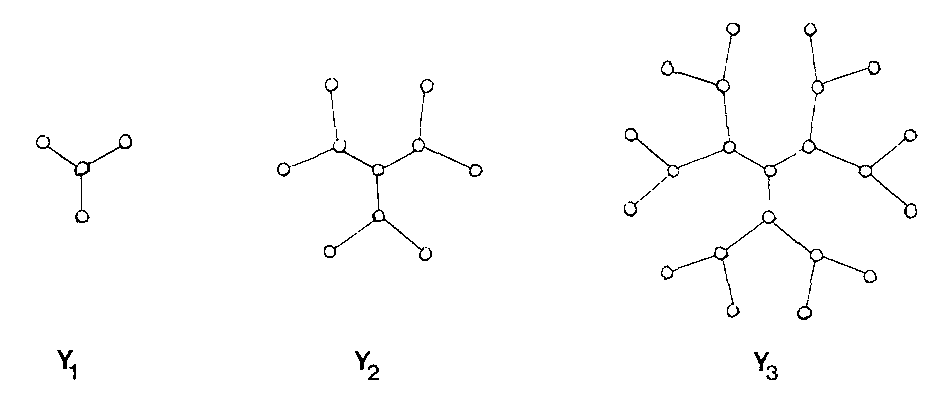
\includegraphics[width=228bp]{figures/fig1}\par
\vspace{14pt}{\small\textsc{Figure} 1}\par}
